
%% bare_conf_compsoc.tex
%% V1.4b
%% 2015/08/26
%% by Michael Shell
%% See:
%% http://www.michaelshell.org/
%% for current contact information.
%%
%% This is a skeleton file demonstrating the use of IEEEtran.cls
%% (requires IEEEtran.cls version 1.8b or later) with an IEEE Computer
%% Society conference paper.
%%
%% Support sites:
%% http://www.michaelshell.org/tex/ieeetran/
%% http://www.ctan.org/pkg/ieeetran
%% and
%% http://www.ieee.org/

%%*************************************************************************
%% Legal Notice:
%% This code is offered as-is without any warranty either expressed or
%% implied; without even the implied warranty of MERCHANTABILITY or
%% FITNESS FOR A PARTICULAR PURPOSE! 
%% User assumes all risk.
%% In no event shall the IEEE or any contributor to this code be liable for
%% any damages or losses, including, but not limited to, incidental,
%% consequential, or any other damages, resulting from the use or misuse
%% of any information contained here.
%%
%% All comments are the opinions of their respective authors and are not
%% necessarily endorsed by the IEEE.
%%
%% This work is distributed under the LaTeX Project Public License (LPPL)
%% ( http://www.latex-project.org/ ) version 1.3, and may be freely used,
%% distributed and modified. A copy of the LPPL, version 1.3, is included
%% in the base LaTeX documentation of all distributions of LaTeX released
%% 2003/12/01 or later.
%% Retain all contribution notices and credits.
%% ** Modified files should be clearly indicated as such, including  **
%% ** renaming them and changing author support contact information. **
%%*************************************************************************


\documentclass[conference,compsoc]{IEEEtran}

% *** CITATION PACKAGES ***
\usepackage[nocompress]{cite}

% *** GRAPHICS RELATED PACKAGES ***
%
\usepackage[pdftex]{graphicx}
% declare the path(s) where your graphic files are
\graphicspath{{../images/}}
% and their extensions so you won't have to specify these with
% every instance of \includegraphics
\DeclareGraphicsExtensions{.jpeg,.png}

% *** MATH PACKAGES ***
\usepackage{amsmath}
% Note that the amsmath package sets \interdisplaylinepenalty to 10000
% thus preventing page breaks from occurring within multiline equations. Use:
%\interdisplaylinepenalty=2500

% *** ALIGNMENT PACKAGES ***
\usepackage{array}

% *** SUBFIGURE PACKAGES ***
\usepackage[caption=false,font=footnotesize,labelfont=sf,textfont=sf]{subfig}

% *** FLOAT PACKAGES ***
%\usepackage{fixltx2e}
%\usepackage{stfloats}
% \usepackage{dblfloatfix}

% *** PDF, URL AND HYPERLINK PACKAGES ***
\usepackage{url}
\usepackage{bm}
%\usepackage{algorithm}
%\usepackage{algorithmic}

% *** Temporary packages ***
\usepackage{lipsum}
\usepackage{pifont}
%\usepackage{xcolor}
%\newcommand\mytodo[1]{\textcolor{red}{#1}}

% correct bad hyphenation here
\hyphenation{op-tical net-works semi-conduc-tor}

\begin{document}

% paper title
\title{Automatic Open Domain Information Extraction\\from Indonesian Text}


% author names and affiliations
% use a multiple column layout for up to three different
% affiliations
\author{
	\IEEEauthorblockN{Yohanes Gultom}
	\IEEEauthorblockA{Faculty of Computer Science\\
	University of Indonesia\\
	Email: yohanes.gultom@ui.ac.id}
	\and
	\IEEEauthorblockN{Wahyu Catur Wibowo}
	\IEEEauthorblockA{Faculty of Computer Science\\
	University of Indonesia\\
	Email: wibowo@cs.ui.ac.id}
}


% make the title area
\maketitle

% As a general rule, do not put math, special symbols or citations
% in the abstract
\begin{abstract}

Availability of big amount digital documents calls for an automatic method to extract information from any text document regardless of domain. Unfortunately, existing open domain information extraction (open IE) systems are not suitable for low-resource language such as Indonesian. This paper introduces a system to extract relation triples from Indonesian text using rule-based triple candidates generator, rule-based token expander and machine-learning-based triple selector. Trained using our 2,344 triples dataset (166 positives \& 2,183 negatives), a Random Forest triple selector model achieves cross-validation score of 0.58 F1 (0.62 precision and 0.58 recall).

\end{abstract}


\section{Introduction}

Open domain information extraction (open IE) is a paradigm that facilitates domain-independent discovery of triple relations from text document\cite{banko2007open}. It extracts relations from sentence in three-values tuples or triples format $(x, r, y)$ where $x$ and $y$ called arguments and $r$ is the relation\cite{etzioni2011open}. In more linguistic term, the arguments are also referred as subject and object while relation are referred as predicate\cite{angeli2015leveraging}. The example of this extraction is described in Figure \ref{fig_example_io_openie}.

As described in Table \ref{table_paradigm_comparison}, unlike traditional information extraction (IE), open IE extracts domain-independent relations from sentence. While it retrieves relations in format of triples similar to knowledge extraction (KE), open IE doesn't follow whole Resource Data Format (RDF) specification\footnote{\url{https://www.w3.org/RDF/}} like KE\cite{auer2007dbpedia} \cite{exner2014refractive}. Although mapping to existing relation schema is required in real word task such as slot filling\cite{angeli2015leveraging}, ontology is not in the scope of open IE research. Open IE has also been reported to be useful for tasks such as question answering\cite{fader2011identifying} and information retrieval\cite{etzioni2011search}. 

\begin{table}[!t]
\renewcommand{\arraystretch}{1.5}
\caption{General comparison between traditional information, open domain information and knowledge extraction}
\label{table_paradigm_comparison}
\centering
\begin{tabular}{|l|>{\centering\arraybackslash}p{1.5cm}|>{\centering\arraybackslash}p{1.5cm}|>{\centering\arraybackslash}p{1.5cm}|}
\hline 
 & \textbf{IE} & \textbf{Open IE} & \textbf{KE} \\ 
\hline 
\textbf{Domain} & Closed & Open & Open \\ 
\hline 
\textbf{Format} & Depends on domain & Triples & RDF Triples \\ 
\hline 
\textbf{Ontology} & Not available & Optional & Mandatory \\ 
\hline 
\end{tabular} 
\end{table}

\begin{figure}
\textbf{Input} \\[0.1cm]
"Sembungan adalah sebuah desa yang terletak di kecamatan Kejajar, kabupaten Wonosobo, Jawa Tengah, Indonesia." \\[0.5cm]
\textbf{Output} \\[0.1cm]
1. (Sembungan, adalah, desa) \\
2. (Sembungan, terletak di, kecamatan Kejajar) \\
\caption{Example of expected input and output of open domain information extraction}
\label{fig_example_io_openie}
\end{figure}

Due to the nature of NLP tasks and heuristics used in open IE system, it is only applicable for a specific language\cite{banko2007open}. So in order to extract open domain information from Indonesian text, a specific system has to be defined for this language. Furthermore, considering the scarcity of Indonesian NLP resources, the system need to effectively utilize them to achieve the objective. Through this paper, we propose a open IE system that addresses these issues.

We propose an open IE system that combine heuristics (rule-based) models and a supervised learning model to extract relation triples from Indonesian text. This approach only requires single manually annotated dataset which is required to train triple selector/classifier. Our objective is to define a baseline system for Indonesian open IE that may be encourage more research in the future.

In general, the contributions from this research are:

\begin{itemize}
\item Open domain information extraction system for Indonesian text
\item Open-source implementation of the system in public repository\footnote{\url{https://github.com/yohanesgultom/id-openie}}
\item Dataset of manually tagged triple candidates
\item Reusable Indonesian NLP pipelines (lemmatizer, part of speech tagger, named-entity recognizer and dependency parser) built by extending Stanford CoreNLP\footnote{\url{https://stanfordnlp.github.io/CoreNLP}} API
\end{itemize}

Further in this paper we will described some of the preeminent related works in open IE, the details about proposed system, experiments using some supervised-learning models as triples selector, analysis of the experiments results, and finally, conclusions and future works of this research.

\section{Related Work}

There has been plenty of works done in the open IE research. Starting from the introduction of open IE along with its first fully-implemented system, TextRunner, which further succeeded by systems built on top of it: ReVerb, R2A2 and Ollie (all from the same research group). The most recent research introduces Stanford OpenIE\footnote{\url{https://nlp.stanford.edu/software/openie.html}} which is an implementation of novel open IE system that outperforms Ollie in TAC-KBP
2013 Slot Filling task\cite{angeli2015leveraging}.

TextRunner was designed for massive size of open-domain web documents by avoiding heavy linguistic tasks and used inverted index to store extraction result\cite{banko2007open}. It generates its own dataset (self-supervised) by using part of speech and dependency features and train a naive bayes classifier to select the triples. It argues that heavy linguistic tasks such as dependency parsing are not scalable to handle million of web documents. Additionally, it also uses redundancy assessor to remove redundant words (stop words, adverbs .etc).

ReVerb is an immediate successor of TextRunner which solves two significant problems in its predecessor: incoherent extractions and uninformative extractions \cite{fader2011identifying}. It is composed of two algorithm: (1) Relation Extraction that extracts relations using syntactical and lexical constraint to solve the problems, and (2) Argument Extraction which retrieve the noun phrases as arguments of the relation. ReVerb takes as input a POS-tagged and NP-chunked and returns a set of relation triples.

R2A2 is a system built to fix argument extraction problem in ReVerb \cite{etzioni2011open}. Instead of using heuristics to extract the arguments, it uses a learning-based system, ArgLearner, that accepts relation and sentence as inputs and returns the first (Arg1) and second arguments (Arg2). ArgLearner extracts the arguments using three classifiers based on REPTree and sequence labeling CRF as described in Figure \ref{fig_arglearner_architecture}.

\begin{figure}
\centering
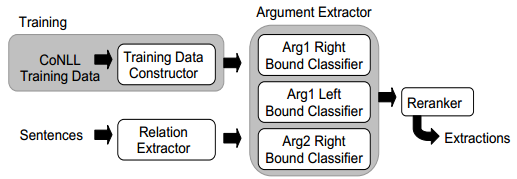
\includegraphics[scale=0.5]{arglearner_architecture}
\caption{ArgLearner architecture training and extraction architecture}
\label{fig_arglearner_architecture}
\end{figure}

Furthermore, Ollie (Open Language Learning for Information Extraction)\cite{schmitz2012open} utilizes ReVerb to learn open pattern templates to guide triples extraction from sentence. Additionally, Ollie does a context analysis to extend the tuples with contextual information in order to improve precision. Its training and extraction architecture is describe in Figure \ref{fig_ollie_architecture}.

\begin{figure}
\centering
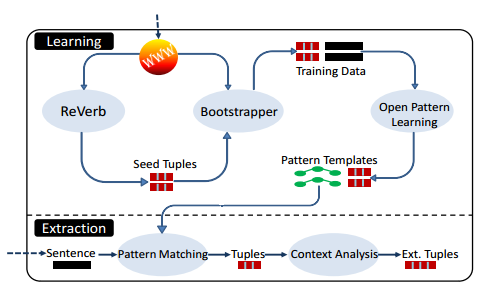
\includegraphics[scale=0.5]{ollie_architecture}
\caption{Ollie labeling and extraction architecture}
\label{fig_ollie_architecture}
\end{figure}

One of the most research proposes new open IE system that replaces the usage of large open patterns in Ollie with a set of fewer patterns for canonically structured sentences and a classifier that learns to extract self-contained clauses from a sentence\cite{angeli2015leveraging}. This system is implemented in Stanford OpenIE which is also integrated in the populer open source suites, Stanford Core NLP.

\section{Proposed System}

Our proposed system also follows the pattern of three-steps\cite{etzioni2011open} method used by open IE system:

\begin{enumerate}

\item \textbf{Label}: sentence are labeled to create a training dataset for the classifier. Although most of the related systems choose to do it automatically (using heuristics or distant supervision)\cite{banko2007open}\cite{etzioni2011open}\cite\cite{schmitz2012open}, we choose to follow the method in recent research\cite{angeli2015leveraging} to manually label our training data to ensure the quality.

\item \textbf{Learn}: train a classifier using the dataset to extract dataset. We use an ensemble model, Random Forest\cite{breiman2001random}, as a classifier since it achieves the best score in our experiment.

\item \textbf{Extract}: use the classifier to extract relations (predicate) and arguments (subjects \& objects) as triples. In our case, we also do token expansion to expand the token into meaningful clause.

\end{enumerate}

As shown in the flowchart Figure \ref{fig_program_flowchart}, our system has three main components:

\begin{figure*}[!t]
\centering
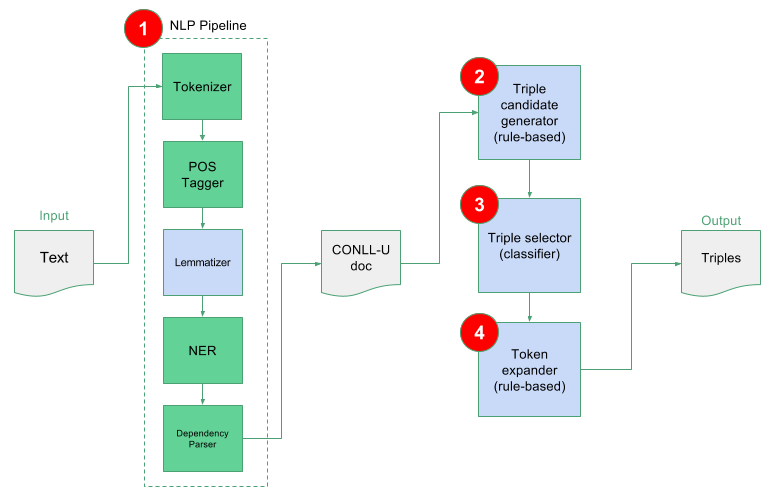
\includegraphics[width=\textwidth]{program_flowchart}
\caption{Indonesian open domain information extraction flowchart}
\label{fig_program_flowchart}
\end{figure*}

%Generally is similar to TextRunner
%
%TextRunner, automatically tag the triples candidates\cite{banko2007open} while we combine automatic candidates generator with manual (human) annotation
%
%These model is based on three-step method of Label, Learn, Extract\cite{etzioni2011open} but use the mix of heuristics and manual labeling

\subsection{NLP Pipeline}

The NLP pipeline is a series of NLP tasks that annotates one or more sentences and saves them in CONLL-U\footnote{\url{http://universaldependencies.org/format.html}} format, a token-based sentence annotation format containing lemma, POS tag, dependency relation and a slot for additional annotation. The model used in each of the NLP tasks in the pipeline are explained below:

\begin{enumerate}

\item \textbf{Tokenizer} \\
We use default tokenizer provided by Stanford Core NLP, \verb|PTBTokenizer|\cite{manningptbtokenizer}, which mimics Penn Treebank 3 tokenizer\footnote{\url{https://catalog.ldc.upenn.edu/LDC99T42}}. While this tokenizer provides many options to modify its behavior, we stick to default configuration that split sentence by whitelines to get the tokens.\\

\item \textbf{Part of Speech Tagger} \\
We trained default Stanford Core NLP \verb|MaxentTagger|\cite{toutanova2003feature} with Indonesian universal POS tag dataset which we convert from dependency parsing dataset\footnote{\url{https://github.com/UniversalDependencies/UD_Indonesian}}. This POS tagger uses Max Entropy (multi-class logistic regression) classifier which yields \textbf{93.68\%} token accuracy and \textbf{63.91\%} sentence accuracy when trained using 5,036 sentences and tested with 559 sentences from the dataset. \\

\item \textbf{Lemmatizer} \\
The lemmatizer used in this pipeline, \verb|IndonesianLemmaAnnotator|, is implemented based on an existing Indonesian rule-based Lemmatizer\cite{suhartono2014lemmatization} with some improvements:

\begin{itemize}
\item Reimplementation in Java language
\item Usage of in-memory database to speed up dictionary lookup
\item Integration with Stanford Core NLP annotator API for reusability
\end{itemize}

This lemmatizer yields \textbf{99\%} accuracy when tested using dataset of 5,638 token-lemma pairs\footnote{\url{https://github.com/davidchristiandy/lemmatizer}}. \\

\item \textbf{Named-Entity Recognizer} \\

Stanford NLP \verb|CRFClassifier|\cite{finkel2005incorporating}, a linear chain Conditional Random Field (CRF) sequence models, is trained using a dataset containing 3,535 Indonesian sentences with 5 entity class: Person, Organization, Location, Quantity and Time. When tested using 426 sentences, this models achieves 0.86 precision, 0.85 recall and \textbf{0.86} F1-score. The dataset itself is a combination between dataset from Faculty of Computer Science, University of Indonesia and a public dataset\footnote{\url{https://github.com/yusufsyaifudin/indonesia-ner}}. \\

\item \textbf{Dependency Parser} \\

We relied on Stanford NLP \verb|nndep.DependencyParser|\cite{chen2014fast}, to annotate dependency relation of each token in the the sentence. We train this transition-based neural network model using a Indonesian universal dependencies dataset of 5,036 sentences and 3,093 Indonesian word embeddings\footnote{\url{https://github.com/yohanesgultom/id-openie/blob/master/data/parser-id.embed}} (vector representation of words). Tested with 559 sentences, this model scores \textbf{70\%} UAS (Unlabeled Attachment Score) and \textbf{46\%} LAS (Labeled Attachment Score).


\end{enumerate}

\begin{figure}
\centering
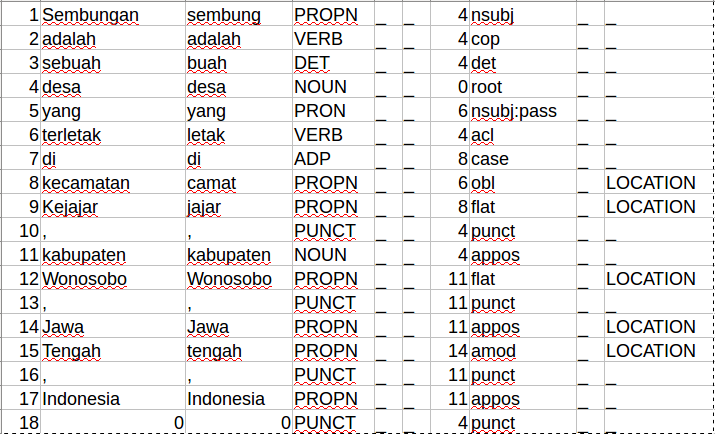
\includegraphics[scale=0.35]{conllu_example}
\caption{CONLL-U Format Example}
\label{fig_conllu_example}
\end{figure}

This pipeline is built by extending Stanford Core NLP classes and packaged as single Java program (JAR). Therefore it can be reused in any other system that require same kind of annotations.

\subsection{Triple Candidates Generator} \label{Triple Candidates Generator}

% Similar to TextRunner Self-Supervised Learner but doesn't automatically label triples

Triple candidates generator is used to extract relation triples candidates from CONLL-U document produced by NLP pipline. It uses a set of rules listed in Table \ref{table_triple_candidate_generation_rules} to extract relations (predicates) and arguments (subjects and predicates) from the sentence. The results of triples extraction are not always the positive or valid relation triples so, unlike TextRunner\cite{banko2007open}, we cannot use them directly as training data for triple selector/classifier.

For example, applying the rules to a annotated sentence in Figure \ref{fig_conllu_example} will generate these 17 triples candidates--where only five of them are valid triples:

\begin{itemize}
\item (Sembungan, adalah, desa) \ding{51}
\item (Sembungan, adalah, terletak)
\item (Sembungan, adalah, kecamatan)
\item (Sembungan, adalah, kabupaten)
\item (Sembungan, adalah, Jawa)
\item (Sembungan, adalah, Tengah)
\item (Sembungan, adalah, Indonesia)
\item (Sembungan, terletak, kecamatan) \ding{51}
\item (Sembungan, terletak, kabupaten) \ding{51}
\item (Sembungan, terletak, Jawa) \ding{51}
\item (Sembungan, terletak, Tengah)
\item (Sembungan, terletak, Indonesia) \ding{51}
\item (desa, terletak, kecamatan)
\item (desa, terletak, kabupaten)
\item (desa, terletak, Jawa)
\item (desa, terletak, Tengah)
\item (desa, terletak, Indonesia)
\end{itemize}

In order to build a training data for the triple selector, we used triple candidates generator to generate 1,611 triple candidates from 42 sentences. From the candidates, we manually labeled 132 positive and 1,479 negative triples which we use to train binary classifier as triple selector in the training phase.

During the extraction phase, triple candidates generator is used in the system to extract unlabeled candidates from CONLL-U document. These unlabeled triples will be labeled by trained triple selector as described in  (referring to flowchart in Figure \ref{fig_program_flowchart}.

% Triple candidate generation rules
\begin{table}[!t]
\renewcommand{\arraystretch}{1.5}
\caption{Triple candidate generation rules}
\label{table_triple_candidate_generation_rules}
\centering
\begin{tabular}{l|p{6cm}}
\hline
\textbf{Type} & \textbf{Condition} \\
\hline
Subject & Token's POS tag is either PROPN, NOUN, PRON or VERB \\
\space & Token is not "yang" nor "adalah" \\
\space & Token's dependency is neither "compound" nor "name" \\
\space & Token's dependency is either "compound" or "name" but separated by more than 2 tokens from its head \\
\hline
Predicate & Token's position is after Subject \\
\space & Token's POS tag is either VERB or AUX \\
\hline
Object & Token's position is after Subject and Predicate \\
\space & Token's POS tag is either PROPN, NOUN, PRON or VERB \\
\space & Token is not "yang" nor "adalah" \\
\space & Token's dependency is neither "compound" nor "name" \\
\space & Token's dependency is either "compound" or "name" but separated by more than 2 tokens from its head \\
\end{tabular}
\end{table}


\subsection{Triple Selector}

Triple selector is a machine learning classifier trained using manually labeled dataset of valid and invalid relation triples. For example, given the input of 17 candidates in Section \ref{Triple Candidates Generator}, the selector will label the five check-marked triples as true and label the rest as false.

We use Random Forest\cite{breiman2001random}, an ensemble methods that aggregate classification results from multiple decision trees, as the model for the classifier. We use the Scikit-Learn\footnote{\url{http://scikit-learn.org}} implementation of Random Forest with following configuration:

\begin{itemize}
\item Decision tree criterion: Gini Impurity
\item Minimum number of samples to split internal node: 5
\item Maximum trees depth: 8
\item Number of trees: 20
\item Maximum features used in each tree: 4 (square root of the number of features)
\item Class weight: balanced (multiplied by the ratio of training samples)
\end{itemize}

As for the features, we use 18 features described in Table \ref{table_models_features} which are based on POS tag, named-entity and dependency relation, instead of shallow syntactic features used by TextRunner or ReVerb\cite{banko2007open}\cite{etzioni2011open}. We encode every nominal features and normalize the whole dataset by removing the mean and scaling to unit variance in order to improve the precision and recall of the classifier.

\begin{table}[!t]
\renewcommand{\arraystretch}{1.5}
\caption{Triple selector features}
\label{table_models_features}
\centering
\begin{tabular}{r|l}
\hline
\textbf{\#} & \textbf{Features} \\
\hline
1 & Subject token's POS tag \\
2 & Subject token's dependency relation \\
3 & Subject token's head POS tag \\
4 & Subject token's named entity \\
5 & Subject token's distance from predicate \\
7 & Subject token's dependency with predicate \\
8 & Predicate token's POS tag \\
9 & Predicate token's dependency relation \\
10 & Predicate token's head POS tag \\
11 & Predicate token's dependents count \\
12 & Object token's POS tag \\
13 & Object token's dependency relation \\
14 & Object token's head POS tag \\
15 & Object token's named entity \\
16 & Object token's dependents count \\
17 & Object token's distance from predicate \\
18 & Object token's dependency with predicate \\
\end{tabular}
\end{table}


\subsection{Token Expander}

Instead of using lightweight noun phrase chunker\cite{banko2007open}, our system uses rule-based token expander to extract relation or argument clauses. It uses heuristics based on syntactical features (POS tag, dependency relation and named-entity) described in Table \ref{table_token_expansion_rules_s_o} and Table \ref{table_token_expansion_rules_p} to determine whether to expand a token to its dependent, ignore the dependent or even remove the token itself. For example, token expander will expand check-marked triples in Section \ref{Triple Candidates Generator} into:

\begin{itemize}
\item (Sembungan, adalah, desa)
\item (Sembungan, terletak di, kecamatan Kejajar)
\item (Sembungan, terletak di, kabupaten Wonosobo)
\item (Sembungan, terletak di, Jawa Tengah)
\item (Sembungan, terletak di, Indonesia)
\end{itemize}

% Token expansion rules for Subject or Object token
\begin{table}[!t]
\renewcommand{\arraystretch}{1.5}
\caption{Token expansion rules for Subject or Object token}
\label{table_token_expansion_rules_s_o}
\centering
\begin{tabular}{r|p{6cm}|l}
\hline
\textbf{\#} & \textbf{Condition for Subject or Object Token} & \textbf{Action} \\
\hline
1 & If dependent's relation to the token  is either “compound”, “name”  or “amod” & Expand \\
2 & If dependent has same named entity as the token & Expand \\
3 & If dependent and the token are wrapped by quotes or double quotes  & Expand \\
4 & If the head is a sentence root & Ignore \\
5 & If dependent's POS tag is CONJ or its form is either “,” (comma) or “/” (slash) & Ignore \\
6 & If dependent's POS tag is either “VERB” or “ADP” & Ignore \\
7 & If dependent has at least one dependent with “ADP” POS tag & Ignore \\
8 & If the first or last token in expansion result has “CONJ” or “ADP” POS tag & Remove \\
9 & If the first or last index of expansion result is an incomplete parentheses symbol & Remove \\
10 & If the last index of expansion result is “yang” & Remove \\
11 & Else & Ignore \\

\end{tabular}
\end{table}

\begin{table}[!t]
\renewcommand{\arraystretch}{1.5}
\caption{Token expansion rules for Predicate token}
\label{table_token_expansion_rules_p}
\centering
\begin{tabular}{r|p{6cm}|l}
\hline
\textbf{\#} & \textbf{Condition for Predicate Token} & \textbf{Action} \\
\hline
1 & If dependent is “tidak” & Expand \\
2 & Else & Ignore \\
\end{tabular}
\end{table}

\section{Experiments}

In this research, we report two experiments. In the first one, we show the performance comparison (precision \& recall) of four classifiers in selecting valid triples from given candidates. While in the second one, we show the performance of our system (using the best classifier and did end-to-end extraction triples from unlabeled document and observed the required time.

In the first experiment, we chose four classifiers each representing unique characteristics:

\begin{enumerate}
	\item Logistic Regression\cite{fan2008liblinear} (linear-model)
	\item Support Vector Machine\cite{chang2011libsvm} (non-linear model)
	\item Multi Layer Perceptron\cite{hinton1989connectionist} (neural network model)
	\item Random Forest\cite{wasserman2015grid} (ensemble model)
\end{enumerate}

The dataset used in the first experiment was manu

\begin{figure}
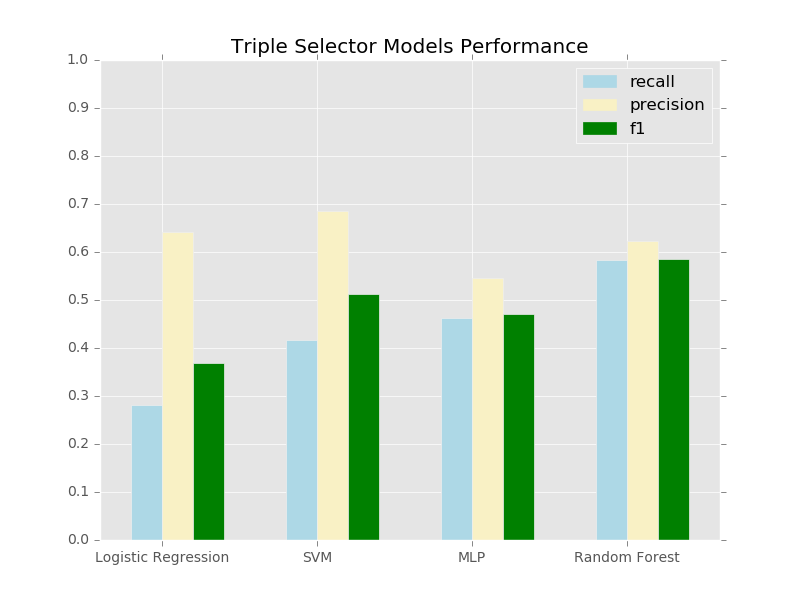
\includegraphics[scale=0.4]{models_performance}
\caption{Triple selector models performance comparison chart}
\label{fig_models_performance}
\end{figure}

\begin{table}[!t]
\renewcommand{\arraystretch}{1.5}
\caption{Triple selector models performance}
\label{table_models_performance}
\centering
\begin{tabular}{l r r r}
\hline
\textbf{Models} & \textbf{P} & \textbf{R} & $\mathbf{F_1}$ \\
\hline
Logistic Regression & 0.64 & 0.28 & 0.36 \\
SVM & \textbf{0.68} & 0.41 & 0.51 \\
MLP & 0.54 & 0.46 & 0.47 \\
Random Forest & 0.62 & \textbf{0.58} & \textbf{0.58} \\
\hline
\end{tabular}
\end{table}

%Our system is quite scalable (faster on bigger document)
%Our system has a comparable speed with TextRunner

\begin{table}[!t]
	\renewcommand{\arraystretch}{1.5}
	\caption{System end-to-end extraction time}
	\label{table_system_extraction_time}
	\centering
	\begin{tabular}{l p{1.2cm} p{1.2cm} p{1.2cm}}
		\hline
		\textbf{Sentences} & \textbf{Triples Extracted} & \textbf{Total Time (s)} & \textbf{Time per Sentence (s)} \\
		\hline
		2 & 7 & 6.1 & 0.800 \\
		138 & 429 & 11.3 & 0.082 \\
		5,593 & 19,403 & 78.6 & 0.014 \\
		\hline
	\end{tabular}
\end{table}

\section{Conclusion}

%Introduces open ie extraction model for Indonesian text
%Provides open-source working implementation of the model

%Future works
%Extract implicit relations in sentence using better heuristics
%Use machine learning model for token expansion
%Estimate confidence level in every phases (NLP pipelines, candidate generator, triple selector, token expander) for following process
%Use better feature extraction using Word2Vec and deep learning
%Optimize system to handle large number of documents

\lipsum[6-7]

% conference papers do not normally have an appendix

% use section* for acknowledgment
%\ifCLASSOPTIONcompsoc
  % The Computer Society usually uses the plural form
%  \section*{Acknowledgments}
%\else
  % regular IEEE prefers the singular form
%  \section*{Acknowledgment}
%\fi

\bibliographystyle{IEEEtran}
\bibliography{../pustaka}

% that's all folks
\end{document}
